% ---------------------------------------------------
% ----- Chapters of the template
% ----- for Bachelor-, Master thesis and class papers
% ---------------------------------------------------
%  Created by C. Müller-Birn on 2012-08-17, CC-BY-SA 3.0.
%  Freie Universität Berlin, Institute of Computer Science, Human Centered Computing. 
%
\chapter{Theoretical background}
\label{chap:background}

Before discussing the design and implementation of the UI editor, it is necessary to provide a brief overview of the applied parts of HCI and the specific context, challenges and Opportunities in which the UI editor was developed.
% 

\section{HCI}
Let me start by concretizing the HCI aspects and why this thesis approaches the area from an not so common standpoint.
\\
Many HCI books (e.g. \cite{Interactiondesign:2019ys} or \cite{LearnHCI:2020ys}) implicitly assume \label{def:Greenfield} Greenfield development,
which ''[...] is in its most distinct form when a new product is created from scratch – a new product or product platform, based on new technology, using new methodology and implemented by people who are new to it all.'' \cite{BrownfieldToGreenfield:2021ys}.
\\
While \cite[p. 392]{Interactiondesign:2019ys} for example mentions \textit{Environmental requirements} and \textit{Technical requirements} as part of the requirement discovery, the descriptions of these terms are more focused on physical limitations or user behaviours and technical requirements are mentioned only once and then not discussed further.
\\\\
\textbf{TODO remove paragraph?}
Another important point for this thesis is the already exisitng and diverse user base of exsiting software in the ecosystem, from Purple Experience Developers over Customer Success Managers to the IT departments of our customers. This made the user research phase quite exiting and provided great value, as there was a lot of detailed input, ideas and whishes from the beginning.
\\\\
Thus, the user research phase started with collecting information about diffrent users, and adapting methods like Moderated observations, interviews and questionaires. I approached this phase with an open mind that it is acceptable if individual methods or applications of them are not successful, from which much can also be learned. As an example, after evaluation and test runs, I decided against Questionaires, because they showed less information content than other methods in this case study.
\\
Evaluationg the outcomes of the research is at least as important as the research itself.
I experimented with diffrent ways to prepare and process the data to to present it more clearly as well as to consider different factors when discussing how to progress with the prototype.

\section{Project specific background}
To understand the usecase and value of the UI Editor, we first have to declare the fundamentals of the environment the editor will be embedded in.
The publishing houses resp. their digital departments (in the following \textit{customer}) purchase the license for an app or website (in the following just \textit{app}, as there is not much difference besides the end medium).
Then, they can import content via multiple ways into the system, or the editors write the content directly inside the tools provided as an Software-As-A-Service (SaaS).

\begin{figure}[h]
  \caption{Use Case diagram showing interactions from publishers, readers and frontend developers with the system}
  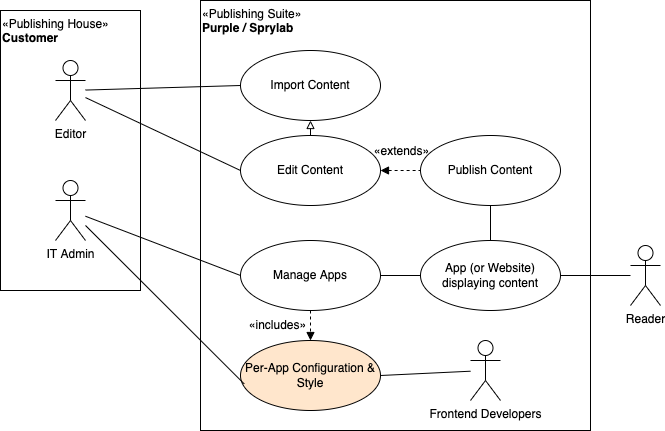
\includegraphics[width=\textwidth]{pics/purple-abstract.drawio.png}
\end{figure}

The UI editor fits into the Use case ''Per App configuration \& style'', with wich mostly Frontend Developers and Project Managers from Sprylab as well as some external customer's IT admins will interact. The goal is to lower the editing burden as much as possible, so that more of the configuration can be handed off to external customers while also improving usability for the developers of the company.
\\
Now that we have established a rough understanding of the environment and usecase the UI editor will be placed in, I want to explain more about the configuration and styling itself.
For that, it is important to understand the Frontend framework Sprylab uses for the delivery to apps and websites. It is called Purple Experience and is a Meta framework build ontop of Angular. The benefit is, that it is completely configurable via JSON files describing the routing, rendering of diffrent components,
connecting data sources (an API abstraction) with those components, loading assets like images and ads, and styling the whole page with CSS.
\\
These configs and assets are stored on an file system called \label{def:DynamicResources} \textit{dynamic resources}.
\\\\
Dynamic resources are individually managed and loaded for every app. This way, on mobile phones the endusers download an native core app, which in turn just downloads the dynamic resources and executes the angular app with the configs provided from the resources.
Similar, when a end user requests a website, the backend server just looks up the dynamic resources matching this Domain or URL, and renders the website using that config.
This way, all customers can share the same server instance(s), or at least don't require extra build artefacts per app.
\\
If you have worked with larger JSON files before, you may recall that they get convoluted quite fast.
Also, manually downloading ZIP files, unpacking them, chaning assets and config files, packing them and uploading and hoping one didn't introduce a typo anywhere is an inefficient an at times quite dangerous workflow.
\\
At Sprylab, there exists an tool called ''Storefront Editor'', which is used as the foundation for this new editor.
In the section about (TODO: LINK!!!) User Research, I will outline the positive aspects and approaches which I reused for the new editor,
as well show the missing features and features the interview candidates noted as confusing, not working or slowing odwn their work.

The following UML sequence diagram displays a typical interaction of a user with the editor; pulling the current version, editing a file and merging the changes.

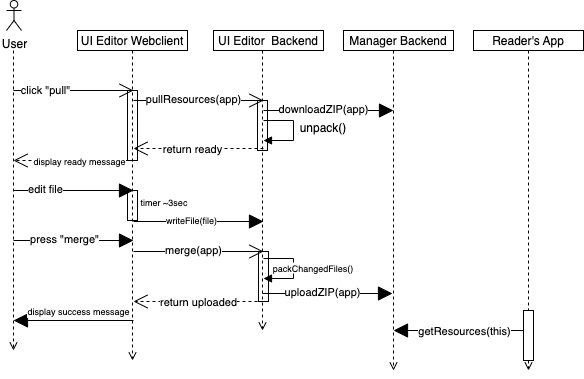
\includegraphics[width=\textwidth]{pics/user-flow.uml.drawio.png}